\documentclass[twocolumn,10pt]{asme2ej}

\usepackage{epsfig} 

\title{%
	Personenzentrisches Projektmanagement\\
	\large 
	- \\
	Einfluss verschiedener Persönlichkeiten auf \\ 
	das Projektmanagement von Data Science Projekten}

\author{Tobias Rohrer
    \affiliation{
	Hochschule Darmstadt\\
	Data Science (Master)\\
    Email: sttorohr@stud.h-da.de
    }	
}

\graphicspath{ {./images/} }
\usepackage[center]{caption}
\usepackage[locale=DE]{siunitx}
\usepackage{hyperref}

\usepackage{listings}
\usepackage{xcolor}
\usepackage{enumitem}
\definecolor{codegreen}{rgb}{0,0.6,0}
\definecolor{codegray}{rgb}{0.5,0.5,0.5}
\definecolor{codepurple}{rgb}{0.58,0,0.82}
\definecolor{backcolour}{rgb}{0.95,0.95,0.92}

\lstdefinestyle{mystyle}{
	backgroundcolor=\color{backcolour},   
	commentstyle=\color{codegreen},
	keywordstyle=\color{magenta},
	numberstyle=\tiny\color{codegray},
	stringstyle=\color{codepurple},
	basicstyle=\ttfamily\footnotesize,
	breakatwhitespace=false,         
	breaklines=true,                 
	captionpos=b,                    
	keepspaces=true,                 
	numbers=left,                    
	numbersep=5pt,                  
	showspaces=false,                
	showstringspaces=false,
	showtabs=false,                  
	tabsize=2
}
\lstset{style=mystyle}
\begin{document}

\maketitle    

%%%%%%%%%%%%%%%%%%%%%%%%%%%%%%%%%%%%%%%%%%%%%%%%%%%%%%%%%%%%%%%%%%%%%%
\begin{abstract}


\end{abstract}

%%%%%%%%%%%%%%%%%%%%%%%%%%%%%%%%%%%%%%%%%%%%%%%%%%%%%%%%%%%%%%%%%%%%%%
\section{Einleitung}
Methoden und Werkzeuge zum Managen von Projekten werden meist anhand des Projektumfangs, Komplexität oder der Klarheit von Anforderungen ausgewählt. Außer acht gelassen wird dabei jedoch, dass sich ein Projektteam aus verschiedenen Persönlichkeiten mit unterschiedlichen Stärken und Schwächen zusammen setzt. Einer der Punkte im Agilen Manifesto lautet sogar "Individuals and interactions over processes and tools" \cite{beck2001agile}. Im Folgenden wird Diskutiert, wie sich verschiedene Projektmanagement-Werkzeuge und Methoden auf die Stärken und Schwächen, sowie auf die Motivation der Persönlichkeiten nach dem DISC-Modell auswirken.

Dazu wird in Abschnitt \ref{sec:1} zunächst das Projektmanagement in Data Science Projekten via Scrum, Kanban und dem Wasserfallmodell, sowie die darin verwendeten Projektmanagement-Werkzeuge gegenüber gestellt.

In Abschnitt \ref{sec:2} werden anschließend die einzelnen Persönlichkeitskategorien nach dem DISC-Modell beschrieben. Außerdem wird diskutiert, wie die Projektmanagement-Methoden und Werkzeuge aus Abschnitt \ref{sec:1} unter Berücksichtigung der Stärken und Schwächen der am Team teilnehmenden Persönlichkeiten eingesetzt werden sollten.


\section{Projektmanagement in Data Science Projekten}\label{sec:1}
Es gibt unzählige Methoden, um Projekte zu verwalten. Im Folgenden werden 3 der meist verbreitetsten kurz beschrieben\footnote{Ausführlichere Beschreibungen der Methoden in den Quellen.}. Anschließend werden die Besonderheiten von Data Science Projekten erläutert und die drei zuvor beschriebenen Methoden im Bezug auf diese Besonderheiten gegenüber gestellt.

\subsection{Wasserfallmodell}
Das Wasserfallmodell lässt sich am besten durch seine sequenziell ablaufenden Phasen charakterisieren. Eine neue Phase wird erst nach erfolgreichem Abschluss der vorgeschalteten Phase gestartet. Zwar bietet das Wasserfallmodell eine gute Übersicht über die Gesamtplanung des Projekts, doch ist es relativ unflexibel gegenüber Veränderungen. \cite{Wasserfall}

\subsection{Agile}
Scrum und Kanan gehören beide zur Gruppe der Agilen Methoden und teilen demnach deren Grundprinzipien. Diese sind im Agile Manifesto gestgehalgen und sind:
- Shortest Path. Reduce Wait times...
\cite{beck2001agile}


\subparagraph{Scrum}
Die Grundiee von Scrum ist die Einteilung des Projektes in Inkremente. Jedes Inkrement wird innerhalb eines sogenannten Sprints bearbeitet und anschließend ausgeliefert. Somit kann kontinuierlich Rückmeldung des Kunden in den Entwicklungsprozess einfließen. In einem Team, das nach Scrum arbeitet gibt es feste Rollen wie den Product Owner, den Scrum Master sowie das Projekt Team. Dem Product Owner obliegt üblicherweise die inhaltliche und dem Scrum Master die organisatorische Verantwortung.

\subparagraph{Kanban}
Angefangene Aufgaben schnellst möglich fertig zu stellen ist eines der zentralen Punkte von Kanban. Um dies zu unterstützten wird üblicherweise ein work in progress (WiP) limit definiert, um sich auf angefangene Aufgaben zu konzentrieren und deren Fertigstellung zu beschleunigen. Dieser Prozess wird auf einem gemeinsamen Kanban Board visualisiert. Hierauf werden die aktuellen Aufgaben, sowie deren Status dargestellt. Ein weiteres Ziel die kontinuierliche Effizienzsteigerung dieses Prozesses.\cite{kanban} Aktualisierungen werden an den Kunden ausgeliefert, sobald Sie fertig sind. In Kanban gibt es keine festen Teamrollen. Üblicherweise wird der Kanban Prozess durch die sogenannte Lead und Cycle Zeit überwacht. Diese misst die Zeit, die eine Aufgabe von der Aufnahme bis zur fertigstellung benötigt. Der Prozess, mit dem das Projektmanagement nach Kanban aufgebaut wird kann sich jederzeit ändern. Im Vergleich zu Scrum kann man Kanban als eher kontinuierliche Methode sehen, wobei Scrum auf feste Inkremente mit definiertem Start und Ende (Sprints) arbeitet.

\subsection{Besonderheiten von Data Science Projekten}
Bei Data Science Projekten ist zu Projektstart oft nicht genau abzuschätzen, ob und in wie fern die festgelegten Ziele mit den verfügbaren Daten erreicht werden können. Dies liegt unter anderem daran, dass die Qualität der zu verarbeitenden Daten fehl eingeschätzt wird. Diese wird in der Praxis eher über statt unterschätzt. Unter Anderem findet deshalb die Auswahl der einzusetzenden Technologien oft erst im laufe des Projektes statt \cite{agile_pm}. Darüber Hinaus können sich die Anforderungen im Laufe des Projektes ändern. Beispielsweise werden durch die Verarbeitung der Daten neue Möglichkeiten vom Entwicklungsteam aber auch von den "Kunden" überhaupt erst erkannt. 

\subsection{Die Auswahl einer passenden Methode}

\begin{figure}
	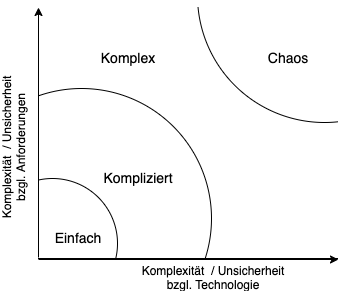
\includegraphics[scale=0.65	]{stacey.png}
	\caption[center]{Die Stacey Matrix angelehnt an \cite{stacey_img}}
	\label{fig:stacey}
\end{figure}

Eine Herausforderung zu beginn vieler Projekte stellt die Wahl einer passenden Projektmanagement Strategie da. Hierbei kann die Stacey Matrix \cite{Stacey2011StrategicMA} unterstützen, indem Projekte in Einfach, Kompliziert, Komplex oder Chaotisch klassifiziert werden (siehe Abbildung \ref{fig:stacey}). Die Klassifizierung wird anhand der Unklarheit und Komplexität der eingesetzten Technologien (Wie wird das Projekt umgesetzt), sowie der Klarheit über die Anforderungen an das Projekt (Was wird in dem Projekt umgesetzt) vorgenommen. Bei einer Klassifizierung im "oberen" komplizierten Bereich bis hin zum Chaotischen Bereich sollten Methoden aus dem Agilen Umfeld, in unserem Fall Kanban oder Scrum eingesetzt werden. Bei einer Klassifizierung als Einfach oder im unteren Komplizierten Bereich kann, muss aber nicht, auch das Wasserfallmodell verwendet werden. Durch die oben beschriebenen Unklarheiten bezüglich der Technologien sowie der Ziele sind die meisten Data Science Projekte in der Stacey Matrix eher ab der komplizierten Stufe einzuordnen. Das Wasserfallmodell ist für die meisten Data Science Projekte wegen der Inflexibilität gegenüber unvorhersehbaren kurzfristigen Abweichungen und Änderungen  eher ungeeignet.

-> Unternehmensstruktur !!

\section{DISG Projektmanagement}\label{sec:2}
Ein Projektteam ist dann effizient, wenn die Teilnehmenden motiviert sind und ihre Stärken voll einsetzen können. Es sollte dabei nicht überraschen, dass Personen unterschiedliche Stärken und Schwächen besitzen und sich durch verschiedene Dinge motivieren lassen. Im Folgenden werden Persönlichkeitstypen nach dem DISG-Modell beschrieben, sowie diskutiert wie sich Stärken, Schwächen und Motivation derer in verschiedenen Projektmanagement-Prozessen verhält.

\subsection{DISG-Modell}
Anhand des DISG-Modells \cite{disc} können Persönlichkeiten in die Bereiche Dominant(D), Initiativ(I), Stetig(S) und Gewissenhaft(G). Eine Persönlichkeit setzt sich meist aus unterschiedlichen Bereichen verschieden stark ausgeprägt zusammen. Mit Hilfe eines DISG-Persönlichkeitstests kann ein Persönlichkeitsprofil erstellt werden. Die verschiedenen Persönlichkeitstypen nach dem DISG-Modell haben typische Stärken und Schwächen, sowie Motivationsfaktoren. 

\subsection{Der Dominante}
Der Dominante  wird vor Allem durch Erfolge und Herausforderungen motiviert. Außerdem genießt der Dominante bei der Bewältigung seiner Aufgaben gerne den Freiraum um Risiken einzugehen und um Entscheidungen zu treffen oder zumindest auf diese einzuwirken. Einer der größten Stärken des Dominanten ist seine Zielorientierte Arbeitsweise, sowie seine sachliche Art des Organisierens. Eine seiner Schwächen, die sich jedoch auch positiv auswirken kann, ist die Ungeduld. Außerdem kann seine direkte Art Konflikte im Team auslösen. Es besteht auch die Gefahr, dass der Dominante seine Autorität überschreitet. Zuletzt laufen Dominante Persönlichkeiten die Gefahr sich bei der Aufgabenplanung zu überschätzen.

\subsubsection{Im Agilen Umfeld}
Eine neue Version des eigenen Produkts an die Kunden auszuliefern kann als Teilerfolg eines Teams interpretiert werden. Das Prinzip einer frühen und kontinuierlichen Auslieferung von funktionierender Software könnte sich daher motivierend auf den Dominanten auswirken. Seine ungeduldige Eigenschaft kann sich sogar positiv darauf auswirken, diesem Prinzip treu zu bleiben. 

Das Prinzip, Projekte um motivierte Personen aufzubauen gibt dem Dominanten den nötigen Freiraum um seine  zielorientierte Arbeitsweise unterzubringen. Durch die enge Zusammenarbeit mit den Stakeholdern kann der Dominante diese von den Ideen des Entwicklungsteams überzeugen, würde aber auch gleichzeitig Gefahr laufen seine Autoritäten zu überschreiten. 

Die Prinzipien der persönlichen Kommunikation, sowie die regelmäßige Reflexion können Probleme  im Team, die durch seine direkte Art zu kommunizieren entstehen, entgegen gewirkt werden.   

\subparagraph{Kanban} kann sich durch das Ziel, angefangene Aufgaben möglichst schnell abzuschließen und dadurch Erfolge zu verbuchen zusätzlich motivierend ausüben und der Ungeduld des Dominanten entgegen wirken. Durch die festgesetzte WiP Grenze wird entgegengewirkt, dass dich der Dominante zu viel auf einmal vornimmt. 

\subparagraph{Scrum} Sprints können sich motivierend auswirken, da sie als Herausforderung angesehen werden können, wobei die erfolgreiche Fertigstellung als Erfolg interpretiert werden kann. Zusätzlich motivierend kann sich die Visualisierung des Fortschrittes eines Sprints auf einem Burndown Chart auswirken. Der Schwäche, sich zu viel vorzunehmen kann in den Sprint Planing Terminen entgegengewirkt werden. Hier ist es üblich, den Aufwand von Aufgaben durch ein sogenanntes Planing Poker mit dem ganzen Entwicklungsteam zu schätzen. Durch die fest eingeplanten Retrospektiven können die Wogen, die durch seine direkte Kommunikation entstehen, direkt geglättet werden. Ist der Hang, seine Autoritäten zu überschreiten stark ausgeprägt, könnte der Scrum Master entgegenwirken.

\subsubsection{Im Wasserfallmodell}
Bei einer Organisation nach dem Wasserfallmodell hingegen, in der vor der Auslieferung noch auf den Abschluss von X gewatet werden muss, könnte sich das durch seine Ungeduld demotivierend auswirken. Demotivierend würden sich auch monotone Routine artige Arbeitsbedingungen auswirken. Außerdem besteht die Gefahr, dass sich der Dominante bei der Anfangsplanung überschätzt und es dadurch zu Fehleinschätzungen im Projektplan kommt. 


\subsection{Die Initiative}
Die Initiative ist in einer Umgebung wo sie Sichtbarkeit und Popularität in der Gruppe erfährt motiviert. Wenn Sie dabei noch Lob und Anerkennung von ihrem Team bekommt verhält sich das zusätzlich motivierend.  Außerdem ist sie ist in einer Umgebung, in der Sie ihre Ideen einbringen und andere von diesen überzeugen kann besonders motiviert. Verstärkt wird das vor Allem durch Bestätigung in ihren Ideen durch die Unterstützung und positivem Feedback Anderer. Durch ihre Kreativität und Impulsivität ist Sie eine gute Ideengeberin. Zu ihren Stärken gehört außerdem, dass sie durch ihre Überzeugungskraft und Optimismus kann Sie motivierend auf andere wirken kann,  wodurch sie oft Popularität erfährt. Diese kann sie nutzen um als Schlichterin in der Gruppe zu fungieren. Ist der Hang zur Impulsivität jedoch stark ausgeprägt,  können aber auch gerne Details bei der Planung oder Durchführung von Aufgaben übersehen werden. Eine weitere Schwäche ist, dass die Initiative schnell die Motivation für bereits angefangene Aufgaben verliert, wobei die Qualität leiden kann.

\subsubsection{Im Agilen Umfeld}
Das Prinzip, dass Projekt um motivierte Personen aufzubauen und zu unterstützen kann sich motivierend auf die Initiative auswirken. Die enge Zusammenarbeit des Entwicklungsteams und der Stakeholder bietet der Initiativen den Raum, um ihre Ideen einzubringen, was sich weiter motivierend auswirkt. Das Prinzip, dass Änderungen in den Anforderungen auch spät im Projektverlauf passieren, ist ebenfalls ganz nach der Initiativen.

\subparagraph{Kanban} bietet den nötigen Freiraum, um der Initiativen die Möglichkeiten zu geben, jederzeit ihre Kreativen Ideen einzubringen. 

\subparagraph{Scrum} Sprints könnten der Initiativen bei einer starken Ausprägung ihrer impulsiven Eigenschaft den Rahmen geben, sich auf angefangene und festgelegte Aufgaben zu konzentrieren und diese in entsprechender Qualität fertig zu stellen. Jedoch könnte die starre Sprintplanung der Initiativen ein Stück weit den Raum nehmen um jederzeit ihre kreativen Ideen einzubringen. Eine feste Definition von Definition of Done kann der potentielle Schwäche entgegen wirken, dass die Qualität unter der geringen Motivation von angefangenen und definierten Aufgaben leidet.

\subsubsection{Im Wasserfallmodell}


\subsection{Fazit}
Zusammenfassend lässt sich sagen, dass die Initiative sich in einem Agilen Umfeld wohl effizienter einsetzen lässt. blablabal


\subsection{Der Stetige}
Der Stetige wird unter Anderem durch die unterstützende Teilnahme an Aufgaben motiviert, ohne dabei aber zwingend als treibende Kraft mitzuwirken. Teammitgliedern zu helfen und dadurch Beziehungen aufzubauen bringt hierbei die Motivation. Eine Anerkennung dieser unterstützenden Art durch das Team wirkt sich hierbei besonders motivierend aus. Zu den Stärken gehört, dass sich der Stetige durch seine empathischen und freundlichen Eigenschaften, sowie der Fähigkeit sich unterzuordnen bestens dafür eignet, um die Kommunikation mit Stakeholdern zu übernehmen. Außerdem nimmt er sich gerne Zeit zuzuhören und nimmt sich auch Probleme anderer an, was ihn zu einem guten Team Player macht. Zu den Schwächen gehört eine gewisse Inflexibilität gegenüber Veränderungen. Des Weiteren besteht die Gefahr, dass sich der Stetige mit Aufgaben überlädt, in der Angst mit einen Nein die Harmonie des Teams zu gefährden. Zuletzt kritisiert der Stetige nicht gerne und wird auch nicht gerne kritisiert.

\subsubsection{Im Agilen}
In Agilen Projekten werden Personen und zwischenmenschliche Interaktionen über Prozesse und Tools angeordnet. Diese Priorisierung kann sich positiv auf die Harmonie im Team auswirken und sich somit motivierend auf den Stetigen auswirken. Eines der Agilen Prinzipien ist die technischen Exzellenz. Diese wird unter Anderem durch sogenannte Code Reviews sicher gestellt. Hierfür bietet sich der Stetige bestens als geduldiger Überprüfer an. Es sollte aber darauf geachtet werden, dass der Stetige berechtigte Kritik anbringt und diese nicht aus Angst die Harmonie zu gefährden zurück hält. 

Responding to Change eher net so.?


\subparagraph{Kanban} hat das Ziel angefangene Aufgaben möglichst schnell abzuschließen. Hierbei kann der Stetige durch seine unterstützende Art behilflich sein und der daraus entstehenden Beziehungen  auch noch Motivation schöpfen. Durch Unterstützende Tätigkeiten können Aufgaben schneller abgeschlossen werden. Außerdem wird durch das gemeinsame arbeiten an Aufgaben das Wissen in einem Team verteilt, wodurch weniger Flaschenhälse entstehen und auch zukünftige Tasks schneller abgearbeitet werden können \cite{kanban}. Eines der Prinzipen von Kanban sieht vor, dass aktuelle Prozesse und Verantwortlichkeiten respektiert und iterativ und stetig angepasst werden. Dies ist für den Stetigen wichtig und eine zu schnelle Veränderung könnte sich demotivierend auswirken. Durch die Verwendung eines Kanban Boards hat der Stetige jederzeit den aktuellen Standes der Aufgaben im Blick, was ihm Sicherheit gibt.

\subparagraph{Scrum} Eine Organisation nach Scrum könnte dem Stetigen durch die Definition fester Rollen und Sprint-Inkremente (Keine Änderungen der Aufgaben innerhalb eines Sprints) die nötige Struktur geben.

\subsubsection{Wasserfallmodell}
Die Planungssicherheit kann sich motivierend auf den Stetigen auswirken.
 
\subsection{Die Gewissenhafte}
Die Gewissenhafte lässt sich vor Allem durch einen hohen Qualitätsstandard, der ihrem perfektionistischen Hang entgegen kommt, motivieren. Bei einem hohen Qualitätsstandard können Fehler ausgeschlossen werden, was wiederum beweist, dass die Gewissenhafte richtig liegt und ihre Aufgaben gründlich durchgeführt hat, was sich weiter motivierend auswirkt. Zu den größten Stärken der Gewissenhaften gehört durch ihr Qualitätsbewusstsein die Gründlichkeit bei der Bearbeitung von Aufgaben. Auch bei den Aufgaben Anderer testet die Gewissenhafte gerne und bringt Verbesserungsvorschläge ein. Ist ihr Qualitätsbewusstsein zu stark ausgeprägt kann dies auch ein Nachteil sein. Dann "verkünstelt" sich die Gewissenhafte gerne.

\subsubsection{Im Agilen}
\subparagraph{Kanban}
In Scurm beispielsweise gibt es eine Klare Struktur wie Aufgaben mit User Stories festgehalten werden usw. ...?
\subparagraph{Scrum}
Beispielsweise bei zu lang und ausführlich gehaltenen nicht faktenbasierenden Diskussionen und Meetings (arbeitet auch gerne mal alleine!). Dabei ist vor Allem bei den in Scrum üblichen Meetings zu achten. Festes Ende der Aufgaben: Entgegenwirken würde hierbei beispielsweise die festgelegte Dauer eines Sprints in Scrum

\subparagraph{Stärken und Schwächen}

\subsection{Im Wasserfallmodell}
Aber auch die Due Dates in Wasserfallmodellen sind hartes ende vong perfektionismus her.. Des weiteren ist die Motivation der Gewissenhaften davon abhängig, in wie weit die Organisation des Projektes sowie Entscheidungen logisch, nachvollziehbar und Faktenbasiert stattfinden. Es kann sich demotivierend auswirken, wenn wichtige Entscheidungen "aus dem Bauch heraus" getroffen werden. In Wasserfallmodellen werden die Aufgaben und der Prozess oft sehr Früh und daher nicht der Realität entsprechend geplant. 

\cite{disc_pm}
\subsection{Teamzusammensetzung}
Bei einem Team also mit überwiegend X und X blablabla.

\section{Beispiele}
Wenn noch Platz ist, könnten hier Beispiele aus der Praxis oder mit fiktiven Personas beschrieben werden.

\section{Fazit}
Hier ein Fazit.

\bibliographystyle{asmems4}

% Here's where you specify the bibliography database file.
% The full file name of the bibliography database for this
% article is asme2e.bib. The name for your database is up
% to you.
\bibliography{pm}

\end{document}
